
\documentclass{../concepts/titul_protokol_p/prepareprotokol} %všechny balíčky pro protokol + titulní strana

\usepackage{graphicx}
\usepackage{newfloat}
\usepackage{caption}
\usepackage{booktabs}
\usepackage{amssymb}
\usepackage{amsmath}
\usepackage{siunitx}
\usepackage{textcomp}
\usepackage{comment}
\usepackage{gensymb}
\usepackage{subcaption}
\usepackage{multirow}
\sisetup{inter-unit-product =$\cdot$}
%\sisetup{separate-uncertainty=true}

\praktikum{III} %číslo praktika (I, II nebo III)
\autor{David Němec} %jméno autora
\datum{31.\,3.\,2026} %datum měření
\cislo{11} %číslo úlohy
\nazev{Stáčení polarizační roviny} %název úlohy

\DeclareFloatingEnvironment[fileext=los, placement={htbp}, name=Obrázek]{schema}

\newcommand{\nobars}{
Chybové úsečky nebyly pro~svou malou velikost pro~přehlednost vykresleny.}

\newcommand{\nohbars}{
Horizontální chybové úsečky nebyly pro~svou malou velikost pro~přehlednost vykresleny.}

\newcommand{\novbars}{
Vertikální chybové úsečky nebyly pro~svou malou velikost pro~přehlednost vykresleny.}

\newcommand{\relative}[1]{
\frac{\sigma_{#1}}{#1}
}
\newcommand{\squared}[1]{
\left( #1 \right)^2
}
\newcommand{\relsqr}[1]{
\squared{\relative{#1}}
%\left( \frac{\sigma_{#1}}{#1} \right)^2
}

\begin{document}
\renewcommand{\figurename}{Graf}
\renewcommand{\refname}{Literatura}
\renewcommand{\today}{\number\day.\,\number\month.\,\number\year}

% add another graphics path to find ZPF.pdf for title page
% now searches for images in ./ and ../concepts/titul_protokol_p/
\graphicspath{{../concepts/titul_protokol_p/}}
\maketitle

% ========================== PRACOVNÍ ÚKOL ============================
\section{Pracovní úkol}
\begin{enumerate}
    \item Změřte závislost stočení polarizační roviny na koncentraci vodního roztoku vzorku sacharidu. 
    Do~grafu vyneste závislost úhlu stočení polarizační roviny lineárně polarizovaného světla na~koncentraci 
    včetně odhadnutých chyb měření. Pro každou koncentraci vypočítejte měrnou stáčivost. Získané hodnoty měrné 
    stáčivosti statisticky zpracujte, tj. vypočítejte střední hodnotu a ~její standardní odchylku.
    \item Změřte Verdetovu konstantu kapalného vzorku. Vyneste do~grafu závislost úhlu stočení polarizační 
    roviny lineárně polarizovaného světla na~magnetické indukci. Pro~každou hodnotu magnetické indukce 
    vypočítejte Verdetovu konstantu. Z~těchto dat vypočtěte střední hodnotu Verdetovy konstanty a~její standardní 
    odchylku.
\end{enumerate}

% ============================= TEORIE ================================ asi hotovo
\vspace{-3mm}
\section{Teorie}

\subsection{Opticky aktivní kapaliny}
Organické látky obsahující asymetrický uhlík (tj. uhlík vázaný na~čtyři různé skupiny) jsou schopné stáčet rovinu
polarizovaného světla. Grupa symetrie takových molekul obsahuje šroubovou osu, podél které se~může šířit jen
kruhově polarizované světlo, proto se~lineárně polarizované světlo při~dopadu na~takovou látku rozloží na~dvě
složky - pravotočivou šířící se rychlostí odpovídající indexu lomu $N_r$ a~levotočivou šířící se~rychlostí
odpovídající $N_l$. V~důsledku asymetrie molekul jsou tyto indexy lomu různé, což vede ke~změně fázového posunu
mezi oběma složkami. Po~výstupu z~látky do~izotropního prostředí se~obě kruhově polarizované složky znovu
sloučí do~lineárně polarizovaného světla, v~důsledku fázového posunu však bude rovina polarizace stočena
o~úhel $\alpha$. Detailní popis a~vysvětlení je v~\cite{studijni}. V~roztoku opticky aktivní látky je~úhel stočení
$\alpha$ úměrný délce dráhy v~látce $d$ a~koncentraci $c$ podle vztahu \cite{studijni}
\begin{equation}
    \label{eq:klasicke_staceni}
    \alpha = \rho c d \,,
\end{equation}
kde $\rho$ je~konstanta úměrnosti nazývaná měrná stáčivost. Její hodnota je specifická pro~každou látku
a~závisí na~vlnové délce světla a~teplotě.

\subsection{Faradayův jev}
I~v~jinak opticky neaktivních látkách může dojít ke~stáčení polarizovaného světla, pokud jsou vloženy do~magnetického
pole. V~důsledku Lorenzovy síly působící na~elektrony, které kmitají kolem jader jako lineární harmonické oscilátory,
dojde k~odlišné interakci elektronů s~elektrickou intenzitou dopadající světelné vlny. Podle \cite{studijni}
se~lineárně polarizované světlo rozloží na~pravotočivou a~levotočivou kruhově polarizovanou složku podobným
způsobem jako v~případě opticky aktivní látky. Indexy lomu obou opačných polarizací se~liší, při~průchodu látkou
dojde k~fázovému posunu mezi složkami a~po~výstupu bude původní lineárně polarizované světlo stočeno o~úhel
$\alpha$. Pro~běžné (nepříliš velké) hodnoty magnetického pole je rozdíl indexů lomu pravotočivé a~levotočivé 
polarizace, a~tím i~úhel stočení, přímo úměrný magnetické indukci vnějšího pole. Pro~úhel $\alpha$ tak bude
platit \cite{studijni}:
\begin{equation}
    \label{eq:faraday_staceni}
    \alpha = V B d \,,
\end{equation}
kde $d$ je opět délka dráhy světla v~látce, $B$ je velikost magnetické indukce a $V$ je Verdetova konstanta 
závislá na~vlastnostech látky a~vlnové délce a~úhlové frekvenci dopadajícího světla.

V~této úloze bylo magnetické pole zprostředkováno solenoidem, přičemž pro~střední hodnotu magnetické
indukce platí přibližný vztah \cite{pokyny}
\begin{equation}
    \label{eq:indukce_na_proudu}
    B = 0.0138 I \,,
\end{equation}
kde $B$ je hodnota magnetické indukce v~jednotkách \unit{\tesla} a $I$ je velikost proudu v~jednotkách \unit{\ampere}.

\subsection{Metoda měření}
Schéma polarimetru použitého pro~určení úhlu stočení lineárně polarizovaného světla je~na~obrázku \ref{sch:polarimetr}.
Jako světelný zdroj při~měření stáčení polarizační roviny roztokem glukózy sloužila rtuťová výbojka s~filtrem
propouštějící spektrální čáru rtuti e o~vlnové délce $\lambda_e = \qty{546.1}{\nano\meter}$ \cite{vlnovedelky}.
Polarizátor v~polostínovém provedení propouští dva lineárně polarizované svazky, jejichž roviny polarizace jsou
od~sebe odchýleny o~malý úhel $\delta$. Po~průchodu vzorkem a~analyzátorem dopadá každý z~obou svazků na~jednu 
polovinu zorného pole dalekohledu. Analyzátor se~pootočí do~takové polohy, kdy budou mít obě poloviny stejný jas
(viz obr. \ref{sch:polostin}),
a na~děleném kruhu se~odečte příslušný úhel $\beta$. Úhel stočení polarizační roviny je pak dán rozdílem
úhlu $\beta$ se~vzorkem o~koncentraci $c$ a~úhlu $\beta_0$ naměřeného bez aktivního vzorku, tj. jen 
s~destilovanou vodou.

Při~měření úhlu stočení vzorkem benzenu v~magnetickém poli byla jako zdroj světla použita sodíková výbojka
s~maximem vyzařování na~vlnové délce $\lambda_D = \qty{589.3}{nm}$ (spektrální čára D) \cite{vlnovedelky}.
Jako zdroj magnetického pole posloužil solenoid zapojený ke~zdroji podle schématu \ref{sch:obvod}. Schéma celé
sestavy je pak na~obrázku \ref{sch:faraday}. Úhel stočení polarizační roviny $\alpha$ je v~tomto případě dán
rozdílem úhlů $\beta$ (s~proudem $I\ne 0$) a~$\beta_0$ (bez proudu).

\begin{schema}[!htbp]
    \centering
    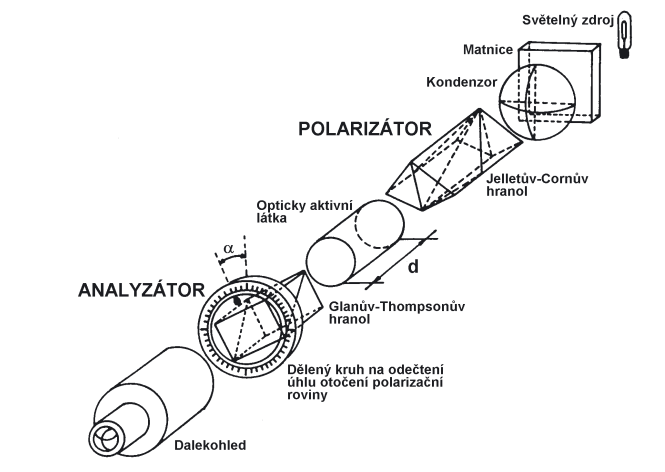
\includegraphics[width=0.7\linewidth]{polarimetr.png}
    \caption{Schéma polarimetru v~polostínovém provedení. \cite{studijni}}
    \label{sch:polarimetr}
\end{schema}

\begin{schema}[!htbp]
    \centering
    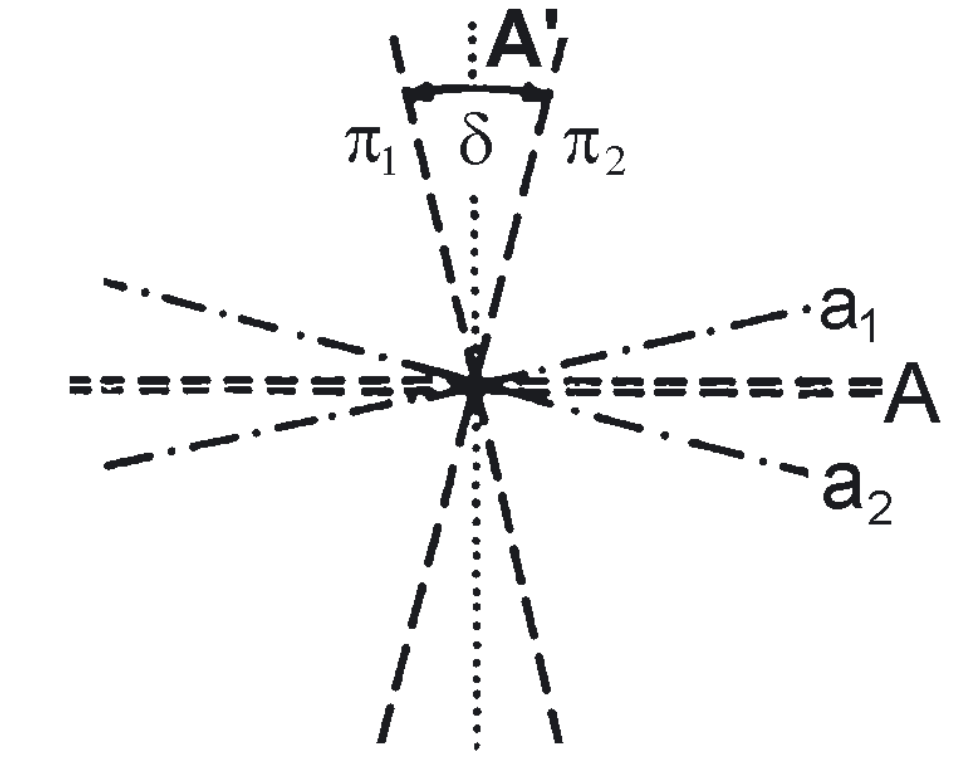
\includegraphics[width=0.4\linewidth]{polostin.png}
    \caption{Princip polostínové metody. Polarizátor propustí dva svazky s~polarizačními rovinami $\pi_1$ a~$\pi_2$.
    Při~nastavení polarizační roviny analyzátoru do~pozice $a_1$ resp. $a_2$, bude v~dalekohledu tmavá polovina
    zorného pole odpovídající svazku $1$ resp. $2$. V~pozici $A$ budou mít obě poloviny zorného pole stejný jas.
    \cite{studijni}}
    \label{sch:polostin}
\end{schema}

\begin{schema}[!htbp]
    \centering
    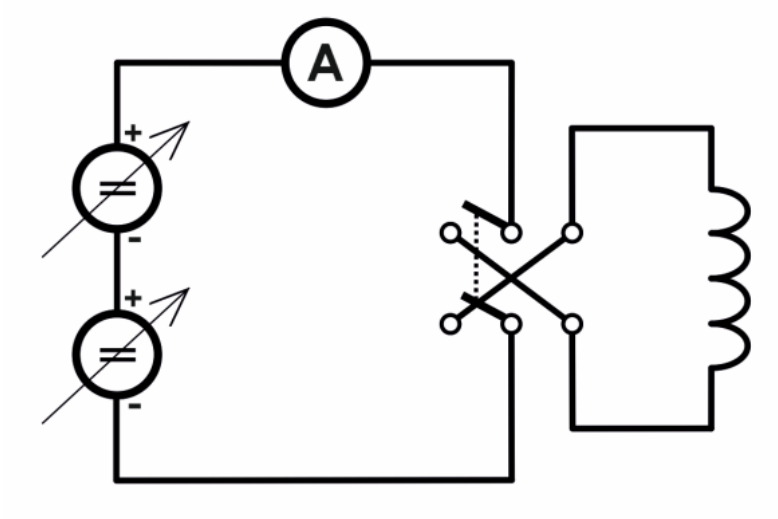
\includegraphics[width=0.4\linewidth]{obvod.png}
    \caption{Schéma zapojení solenoidu. \cite{pokyny}}
    \label{sch:obvod}
\end{schema}

\begin{schema}[!htbp]
    \centering
    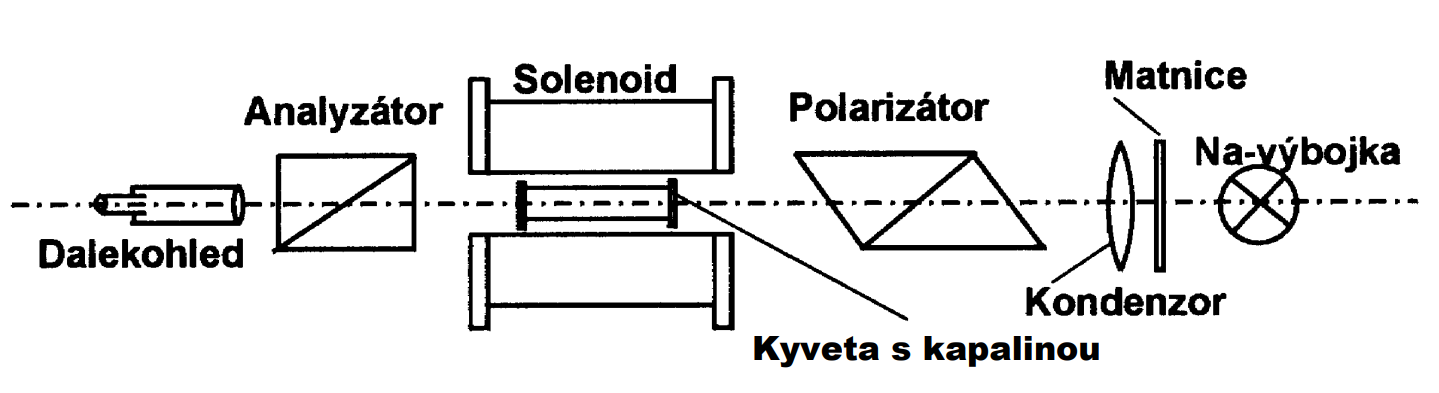
\includegraphics[width=0.6\linewidth]{faraday.png}
    \caption{Sestava pro~určení Verdetovy konstanty benzenu. \cite{pokyny}}
    \label{sch:faraday}
\end{schema}


\subsection{Měřicí přístroje a jejich nejistoty}
\begin{enumerate}
    \item \textbf{Dělená kruhová stupnice polarimetru}:
    
    Pro~měření stočení polarizační roviny roztokem glukózy a~vzorkem benzenu byly použity dva různé polarimetry.
    Z~jejich dělené stupnice byl však odečítán úhel se~stejnou přesností, proto je uvádím dohromady.
    Nejistotu určení úhlu na~stupnici (nejistota typu B) odhaduji jako velikost nejmenšího dílku, tedy
    $\sigma_{\beta,B} = 0.01\,\degree$.

    \item \textbf{Dávkovací pipeta Vitrum}:
    
    Pipetou byl odměřován objem glukózy a~destilované vody pro~přípravu roztoků o~různých koncentracích. Relativní
    nejistotu pipetovaného objemu jsem určil v~minulém semestru v~úloze 26 jako $\eta_V = 1.6\,\%$.

    \item \textbf{Multimetr Fluke}:
    
    Multimetrem byl měřen stejnosměrný proud procházející solenoidem. Ze~specifikací přístoje je nejistota
    proudu na~rozsahu \qty{10}{A} $0.2\,\%$ z~měřené hodnoty + $0.01\,\%$ z~rozsahu.

    \item \textbf{Termohygrobarometr Commeter C4130}:
    
    Přístrojem byla změřena teplota okolí během experimentu, nejistota teploty je ze~specifikací přístroje $0.4\,\degree \mathrm{C}$.

\end{enumerate}


% ======================== VÝSLEDKY MĚŘENÍ ===========================
\section{Výsledky měření}

% ======================== glukóza, asi hotovo
\subsection{Stáčení roviny polarizace roztokem glukózy}

Teplota okolí byla změřena jako \qty{22.6(4)}{\degree C}.

Nejprve bylo nutné odhadnout nejistotu určení úhlu $\beta$ na~stupnici polarimetru, jelikož přesnost dělené
stupnice bude jistě větší než~přesnost nastavení dvou polovin zorného pole dalekohledu na~stejný jas, případně
než~přesnost koncentrace namíchaných roztoků. Proto byl vzorek o~koncentraci \qty{100}{g \per l} namíchán třikrát
a~pro~každý z~nich bylo provedeno pět měření úhlu $\beta$. Naměřené hodnoty jsou uvedeny v~tabulce 
\ref{tab:glukoza_nejistota}. Průměr pro~koncentraci \qty{100}{g \per l} je $\overline{\beta} = \qty{4.3}{\degree}$ 
a~standarní nejistota (nejistota jednoho měření) je $\sigma_{\beta} = \qty{0.2}{\degree}$. Ta byla 
vypočtena podle vztahu \cite{englich}
\begin{equation}
    \label{eq:sigma_beta_glukoza}
    \sigma_{\beta} = \sqrt{ \frac{1}{14} \sum_{i=1}^{15} \left( \beta_i - \overline{\beta} \right)^2 } \,.
\end{equation}
Její hodnota byla použita jako odhad nejistoty určení úhlu $\beta$ pro~všechna ostatní měření s~roztoky glukózy,
jelikož experimentátor i~světelné podmínky zůstaly nezměněny.

\begin{table}[!htbp]
\centering
\caption{Úhel na stupnici polarimetru pro třikrát namíchaný vzorek o~koncentraci 
\qty{100}{g \per l} pro~zjištění nejistoty úhlu.}
\begin{tabular}{c|ccc}
 \toprule
  & provedení 1 & provedení 2 & provedení 3 \\
 \midrule
 číslo měření & $\beta\, (\mathrm{\degree})$ & $\beta\, (\mathrm{\degree})$ & $\beta\, (\mathrm{\degree})$ \\
 \midrule
 $1$ & $4.52$ & $4.43$ & $3.94$ \\
 $2$ & $4.42$ & $4.55$ & $4.13$ \\
 $3$ & $4.34$ & $4.40$ & $4.17$ \\
 $4$ & $4.43$ & $4.51$ & $4.06$ \\
 $5$ & $4.48$ & $4.27$ & $3.93$ \\
 \midrule
 \midrule
 \multicolumn{2}{c}{průměr: $4.3$} \vline & \multicolumn{2}{c}{standarní nejistota: $0.2$} \\
 \bottomrule
\end{tabular}
\label{tab:glukoza_nejistota}
\end{table}

Následně byly proměřeny ostatní roztoky o~vyšších koncentracích, ale také vzorek čisté destilované vody. 
Úhel stočení $\alpha$ byl určen jako rozdíl úhlu $\beta$ od~úhlu $\beta_0$ naměřeného pro~destilovanou vodu:
\begin{equation}
    \label{eq:alfa_glukoza}
    \alpha = \beta - \beta_0
\end{equation}
a jeho nejistota jako \cite{englich}
\begin{equation}
    \label{eq:sigma_alfa_glukoza}
    \sigma_{\alpha} = \frac{\sqrt{2}}{2} \sigma_{\beta} \,.
\end{equation}
Měrná stáčivost $\rho$ pro~každý roztok glukózy byla určena z~rovnice (\ref{eq:klasicke_staceni}), přičemž během 
měření byla použita kyveta 
o~délce $d_1 = \qty{1}{dm}$. Nejistota $\rho$ byla určena jako \cite{englich}
\begin{equation}
    \label{eq:sigma_rho}
    \sigma_{\rho} = \rho \sqrt{ \relsqr{\alpha} + \relsqr{c}}
\end{equation}
nejistotu délky $d_1$ neuvažuji. Nejistota koncentrace je dána nejistotou pipetovaného objemu glukózy a~celkového
objemu, podle \cite{englich} bude platit:
\begin{equation}
    \label{eq:sigma_c}
    \sigma_c = \sqrt{2} c \,\eta_V \doteq 0.023 \cdot c \,.
\end{equation}

Hodnoty úhlů $\alpha$, $\beta$ a~měrné stáčivosti $\rho$ pro~měřené vzorky
jsou uvedeny v~tabulce \ref{tab:glukoza}, hodnota úhlu $\beta$ pro~koncentraci \qty{100}{g \per l} je vzatá
z~tabulky \ref{tab:glukoza_nejistota}. Z~měrných stáčivostí vzorků o~nenulové koncentraci byla vypočtena
jejich střední hodnota $\overline{\rho}$, přičemž její nejistota je dána vztahem \cite{englich}:
\begin{equation}
    \label{eq:sigma_mean_rho}
    \sigma_{\overline{\rho}} = \sqrt{ \sigma_{\rho, B}^2 + \sigma_{\rho,A}^2 } = \sqrt{ \sigma_{\rho, B}^2 + 
        \frac{1}{4\cdot 5} \sum_{i=1}^{5} \left( \rho_i - \overline{\rho} \right)^2 } \,,
\end{equation}
kde $\sigma_{\rho, B}$ je průměrná nejistota měrné stáčivosti jednotlivých vzorků a~$\sigma_{\rho, A}$ je standardní
nejistota aritmetického průměru měrné stáčivosti.

\begin{table}[!htbp]
\centering
\caption{Úhel na stupnici polarimetru a měrná stáčivost roztoků glukózy o~různých koncentracích.}
\begin{tabular}{cccc}
 \toprule
 $c\, (\mathrm{g/l})$ & $\beta\, (\mathrm{\degree})$ & $\alpha\, (\mathrm{\degree})$ & $\rho\, (\mathrm{\degree dm^2 g^{-1}})$ \\
 \midrule
 $0.0(0)$ & $-0.7(2)$ & $0.0(3)$ & --- \\
 $100(2)$ & $4.3(2)$ & $5.0(3)$ & $0.050(3)$ \\
 $200(5)$ & $9.5(2)$ & $10.2(3)$ & $0.0511(19)$ \\
 $300(7)$ & $15.0(2)$ & $15.6(3)$ & $0.0521(15)$ \\
 $400(9)$ & $20.2(2)$ & $20.9(3)$ & $0.0523(14)$ \\
 $500(11)$ & $25.4(2)$ & $26.1(3)$ & $0.0522(13)$ \\
 \midrule
 \midrule
 \multicolumn{3}{r}{průměr} & $0.052(2)$ \\
 \bottomrule
\end{tabular}
\label{tab:glukoza}
\end{table}

Datové body závislosti úhlu $\beta$ na~koncentraci $c$ jsou zobrazeny v~grafu \ref{fig:glukoza}. Pro~větší
přesnost určení měrné stáčivosti jimi byla
proložena lineární funkce ve~tvaru $\beta = \tilde{\rho} c + \beta_0$ (díky tomu, že $d_1 = \qty{1}{dm}$, 
je směrnice přímky číselně přímo rovna měrné stáčivosti $\tilde{\rho}$). Metodou nejmenších čtverců pomocí
funkce \texttt{curve\_fit} knihovny \texttt{scipy.optimize} byly určeny koeficienty 
$\tilde{\beta}_0 = \qty{-0.83(15)}{\degree}$ a~$\tilde{\rho} = \qty{0.0525(5)}{ \degree dm^2 g^{-1} }$. 
% Nejistoty získané 
% z~fitu (označené vlnovkou) byly opraveny o~nejistoty $\sigma_{\beta}$ a~$\sigma_c$ podle vztahu \cite{englich}
% \begin{equation}
%     \label{eq:combined_sigma_beta_glukoza}
%      \sigma_{\tilde{\beta}_0} = \sqrt{ \tilde{\sigma}_{\tilde{\beta}_0}^2 + \sigma_{\beta}^2 } \,,  
% \end{equation}
% \begin{equation}
%     \label{eq:combined_sigma_rho_glukoza}
%     \sigma_{\tilde{\rho}} = \sqrt{ \relsqr{\beta} + \relsqr{c} } \,.
% \end{equation}

\begin{figure}
    \centering
    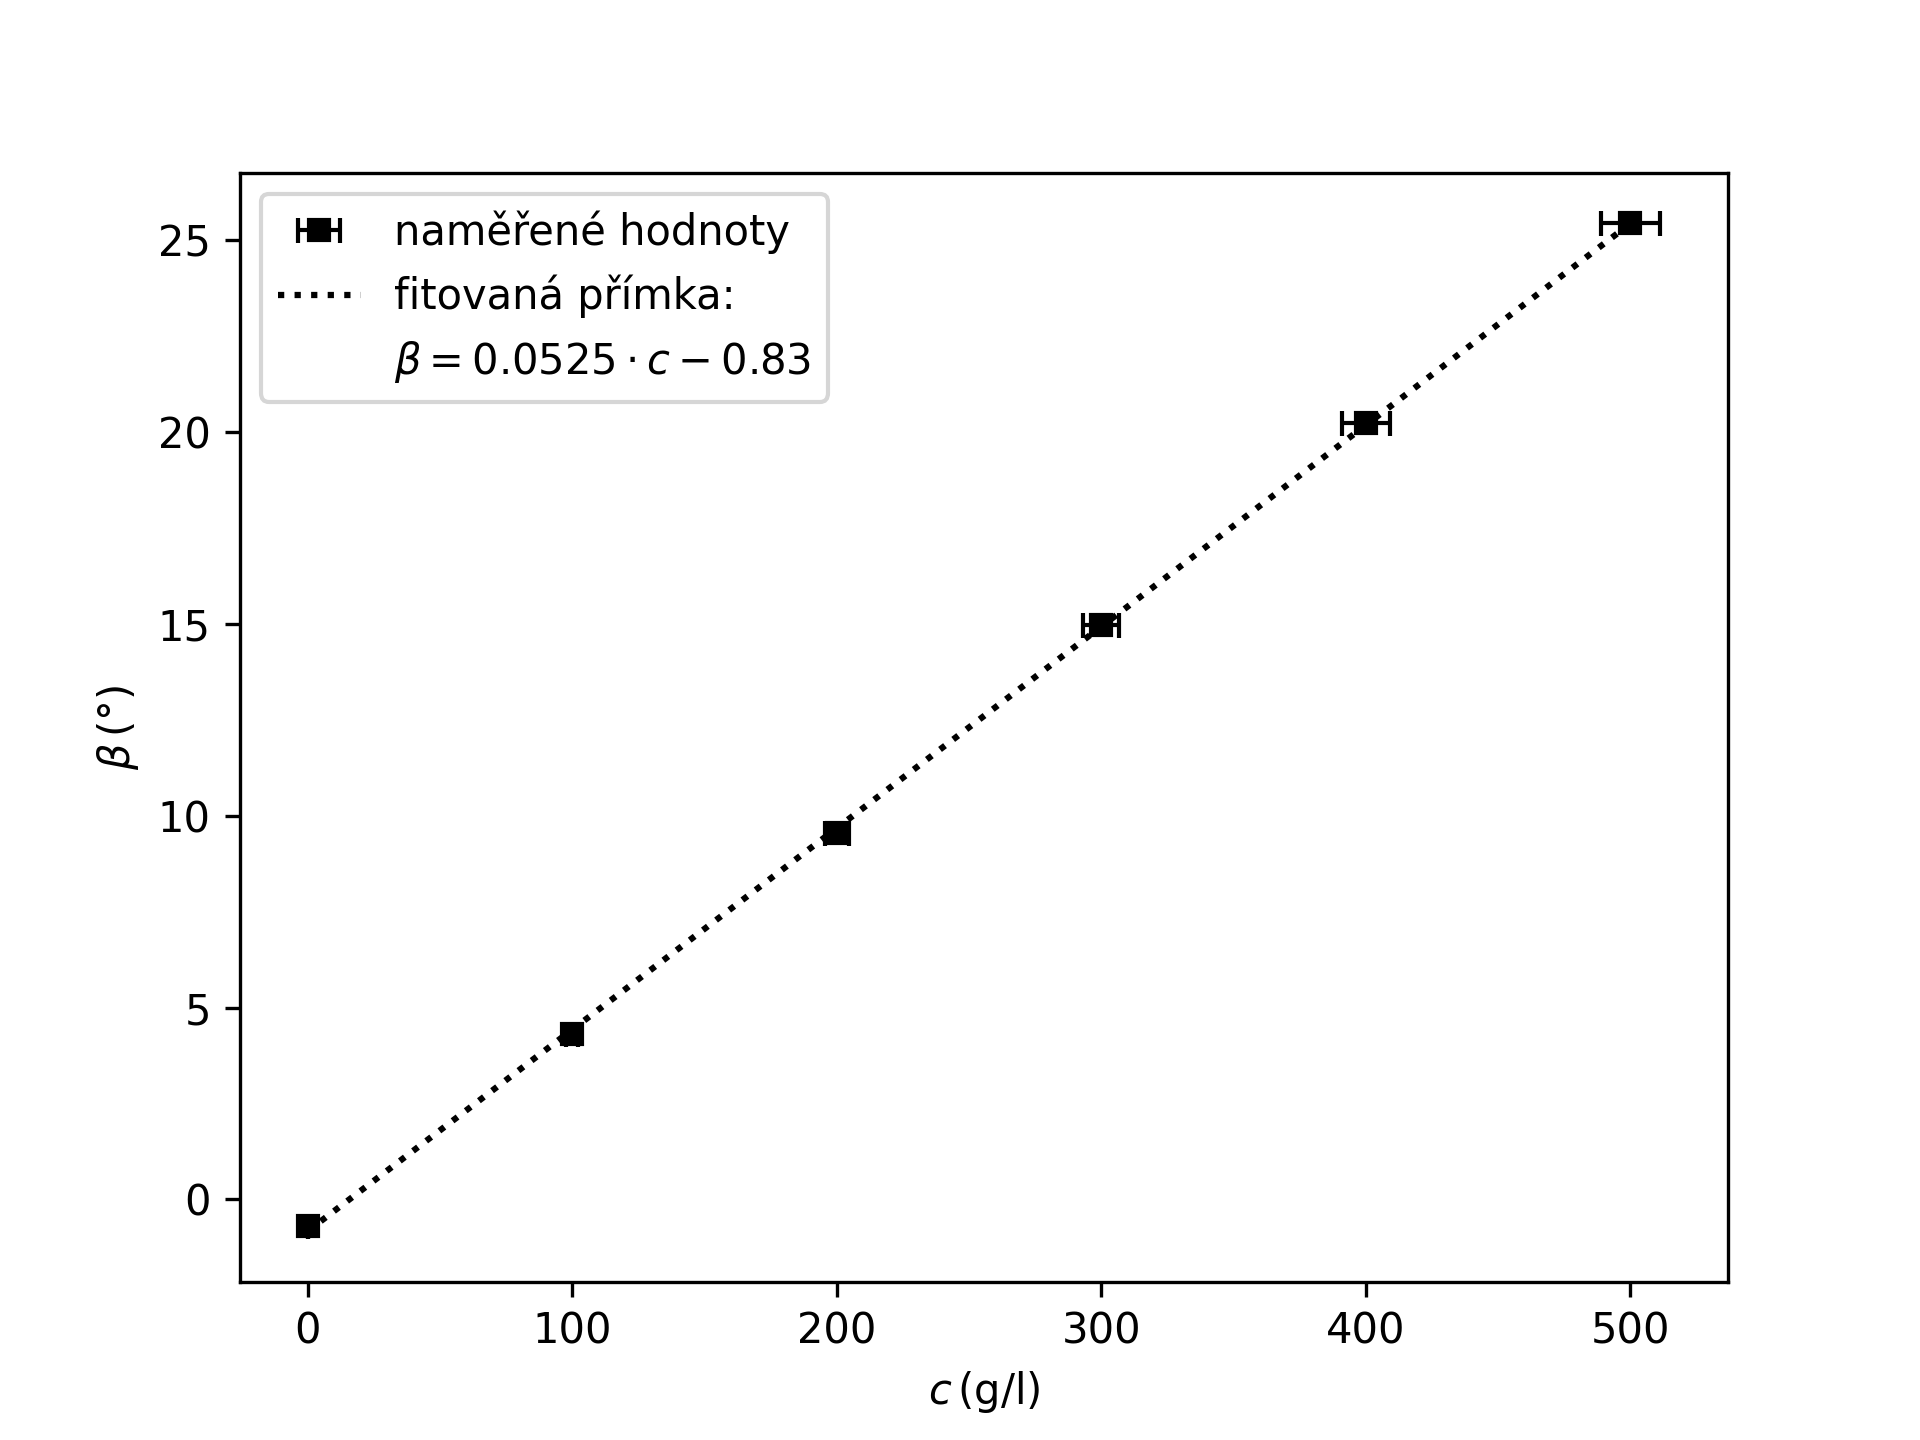
\includegraphics[width=0.6\linewidth]{glukoza.png}
    \caption{Závislost úhlu $\beta$ na~stupnici polarimetru na~koncentraci roztoků glukózy.\novbars}
    \label{fig:glukoza}
\end{figure}

% ======================= benzen asi hotovo
\subsection{Stáčení roviny polarizace vzorkem benzenu v magnetickém poli solenoidu}

Uvnitř solenoidu o~délce \qty{25}{cm} s~3045 závity byla umístěna kyveta se~vzorkem benzenu o~délce 
$d_2 = \qty{2}{dm}$ \cite{pokyny}. V~závislosti na~proudu tekoucím solenoidem, a tím na~magnetické indukci solenoidu
dané vztahem (\ref{eq:indukce_na_proudu}), byl proměřován úhel stáčení polarizační roviny lineárně polarizovaného
světla ze~sodíkové výbojky. Pro~určení nejistoty úhlu byl pro~každý ze~tří vybraných proudů (\qty{-2}{A}, \qty{-1}{A}
a~\qty{1}{A}) pětkrát odečten úhel na~polarimetru při~nastavení obou polovin zorného pole dalekohledu na~stejný jas.
Naměřené hodnoty jsou uvedeny v~tabulce \ref{tab:benzen_nejistota}. Pro~každý ze~tří proudů byl vypočten průměr
a~také nejistota jednoho měření podle vztahu \cite{englich}
\begin{equation}
    \label{eq:sigma_beta_benzen}
    \sigma_{\beta} = \sqrt{ \frac{1}{4} \sum_{i=1}^{5} \left( \beta_i - \overline{\beta} \right)^2 } \,.
\end{equation}
Nejistoty vychází pro~všechny tři proudy stejně, i~pro~ostatní hodnoty (světelné podmínky ani experimentátor 
se~nezměnil) proto budu uvažovat nejistotu určení
úhlu na~stupnici polarimetru $\sigma_\beta = 0.03 \,\degree$.

Dále bylo měřeno stáčení polarizační roviny vzorku benzenu v~magnetickém poli v~rozsahu proudů od~\qty{0}{A} 
do~\qty{3}{A} s~krokem \qty{0.5}{A}, a~to pro~oba směry
proudu. Z~úhlu na~polarimetru $\beta$ byl vypočten úhel stočení polarizační roviny $\alpha$ podle rovnice 
(\ref{eq:alfa_glukoza}), kde úhel $\beta_0$ odpovídá nulovému proudu, a~nejistota úhlu stočení je daná vztahem 
(\ref{eq:sigma_alfa_glukoza}).
Indukce byla vypočtena ze~vztahu (\ref{eq:indukce_na_proudu}) a~její nejistota podle \cite{englich}
jako
\begin{equation}
    \label{eq:sigma_indukce}
    \sigma_B = B \relative{I} \,.
\end{equation}
Pro~každou hodnotu indukce byla z~rovnice (\ref{eq:faraday_staceni}) vypočtena Verdetova konstanta vzorku
a~její nejistota jako \cite{englich}
\begin{equation}
    \label{eq:sigma_verdet}
    \sigma_V = V \sqrt{ \relsqr{\alpha} + \relsqr{B}} \,,
\end{equation}
přičemž nejistotu délky kyvety $d_2$ neuvažuji.

Naměřené hodnoty stočení polarizační roviny a~příslušné Verdetovy konstanty jsou uvedeny v~tabulce 
\ref{tab:benzen}. Z~hodnot Vertovy konstanty byl vypočten aritmetický průměr $\overline{V}$ a~jeho nejistota jako
\begin{equation}
    \label{eq:sigma_V_mean}
    \sigma_{\overline{V}} = \sqrt{ \frac{1}{11 \cdot 12} \sum_{i=1}^{12} \left( V_i - \overline{V} \right)^2 } \,.
\end{equation}
Závislost úhlu na~polarimetru na~magnetické
indukci je vykreslena v~grafu \ref{fig:benzen}. Pro~větší přesnost Verdetovy konstanty byla datovými body proložena lineární závislost ve~tvaru
$\beta = k \cdot B + \beta_0$, kde $d_2 = \qty{2}{dm}$. Metodou nejmenších čtverců pomocí funkce \texttt{curve\_fit} 
byly určeny koeficienty $k = \qty{99.2(6)}{\degree T^{-1}}$ a~$\beta_0 = \qty{11.948(14)}{\degree}$.
Verdetova konstanta byla ze~směrnice fitu $k$ určena podle vztahu
\begin{equation}
    \label{eq:V_from_fit}
    \tilde{V} = \frac{k}{d_2}
\end{equation}
a~její nejistota jako
\begin{equation}
    \label{eq:sigma_V_from_fit}
    \sigma_{\tilde{V}} = \tilde{V} \relative{k} \,.
\end{equation}
Z~lineárního fitu tedy vychází Verdetova konstanta $\tilde{V} = \qty{49.6(3)}{\degree T^{-1} dm^{-1}}$.

\begin{table}[!htbp]
\centering
\caption{Úhel na stupnici polarimetru pro tři různé proudy procházející solenoidem (pro~zjištění
nejistoty úhlu)}
\begin{tabular}{cccc}
 \toprule
 & $I = \qty{-1.998(5)}{A}$ & $I = \qty{-0.997(3)}{A}$ & $I = \qty{1.006(3)}{A}$ \\
 \midrule
 číslo měření & $\beta\, (\mathrm{\degree})$ & $\beta\, (\mathrm{\degree})$ & $\beta\, (\mathrm{\degree})$ \\
 \midrule
 $1$ & $9.23$ & $10.54$ & $13.32$ \\
 $2$ & $9.20$ & $10.57$ & $13.36$ \\
 $3$ & $9.23$ & $10.62$ & $13.37$ \\
 $4$ & $9.27$ & $10.61$ & $13.31$ \\
 $5$ & $9.20$ & $10.58$ & $13.34$ \\
 \midrule
 \midrule
 průměr & $9.23(3)$ & $10.58(3)$ & $13.34(3)$ \\
 \bottomrule
\end{tabular}
\label{tab:benzen_nejistota}
\end{table}

\begin{table}[!htbp]
\centering
\caption{Úhel na stupnici polarimetru, příslušný úhel stočení polarizační roviny a Verdetova konstanta
vzorku benzenu pro~různé hodnoty proudu resp. magnetické indukce solenoidu.}
\begin{tabular}{ccccc}
 \toprule
 $I\, (\mathrm{A})$ & $B\, (\mathrm{T})$ & $\beta\, (\degree)$ & $\beta\, (\degree)$ & $V\, (\mathrm{\degree T^{-1} dm^{-1}})$ \\
 \midrule
 $-2.979(7)$ & $-0.04111(10)$ & $7.85(3)$ & $-4.02(4)$ & $48.9(5)$ \\
 $-2.494(6)$ & $-0.03442(8)$ & $8.60(3)$ & $-3.27(4)$ & $47.5(6)$ \\
 $-1.996(5)$ & $-0.02754(7)$ & $9.26(3)$ & $-2.61(4)$ & $47.4(7)$ \\
 $-1.512(4)$ & $-0.02087(6)$ & $9.85(3)$ & $-2.02(4)$ & $48.4(10)$ \\
 $-1.003(3)$ & $-0.01384(4)$ & $10.54(3)$ & $-1.33(4)$ & $48.0(15)$ \\
 $-0.505(2)$ & $-0.00697(3)$ & $11.23(3)$ & $-0.64(4)$ & $46(3)$ \\
 $0.000(1)$ & $0.00000(2)$ & $11.87(3)$ & $0.00(4)$ & --- \\
 $0.497(2)$ & $0.00686(3)$ & $12.67(3)$ & $0.80(4)$ & $58(3)$ \\
 $1.013(3)$ & $0.01398(4)$ & $13.32(3)$ & $1.45(4)$ & $51.9(15)$ \\
 $1.502(4)$ & $0.02073(6)$ & $14.08(3)$ & $2.21(4)$ & $53.3(10)$ \\
 $2.006(5)$ & $0.02768(7)$ & $14.63(3)$ & $2.76(4)$ & $49.9(7)$ \\
 $2.491(6)$ & $0.03438(8)$ & $15.35(3)$ & $3.48(4)$ & $50.6(6)$ \\
 $2.986(7)$ & $0.04121(10)$ & $16.08(3)$ & $4.21(4)$ & $51.1(5)$ \\
 \midrule
 \midrule
 \multicolumn{4}{r}{průměr} & $50(1)$ \\
 \bottomrule
\end{tabular}
\label{tab:benzen}
\end{table}

\begin{figure}
    \centering
    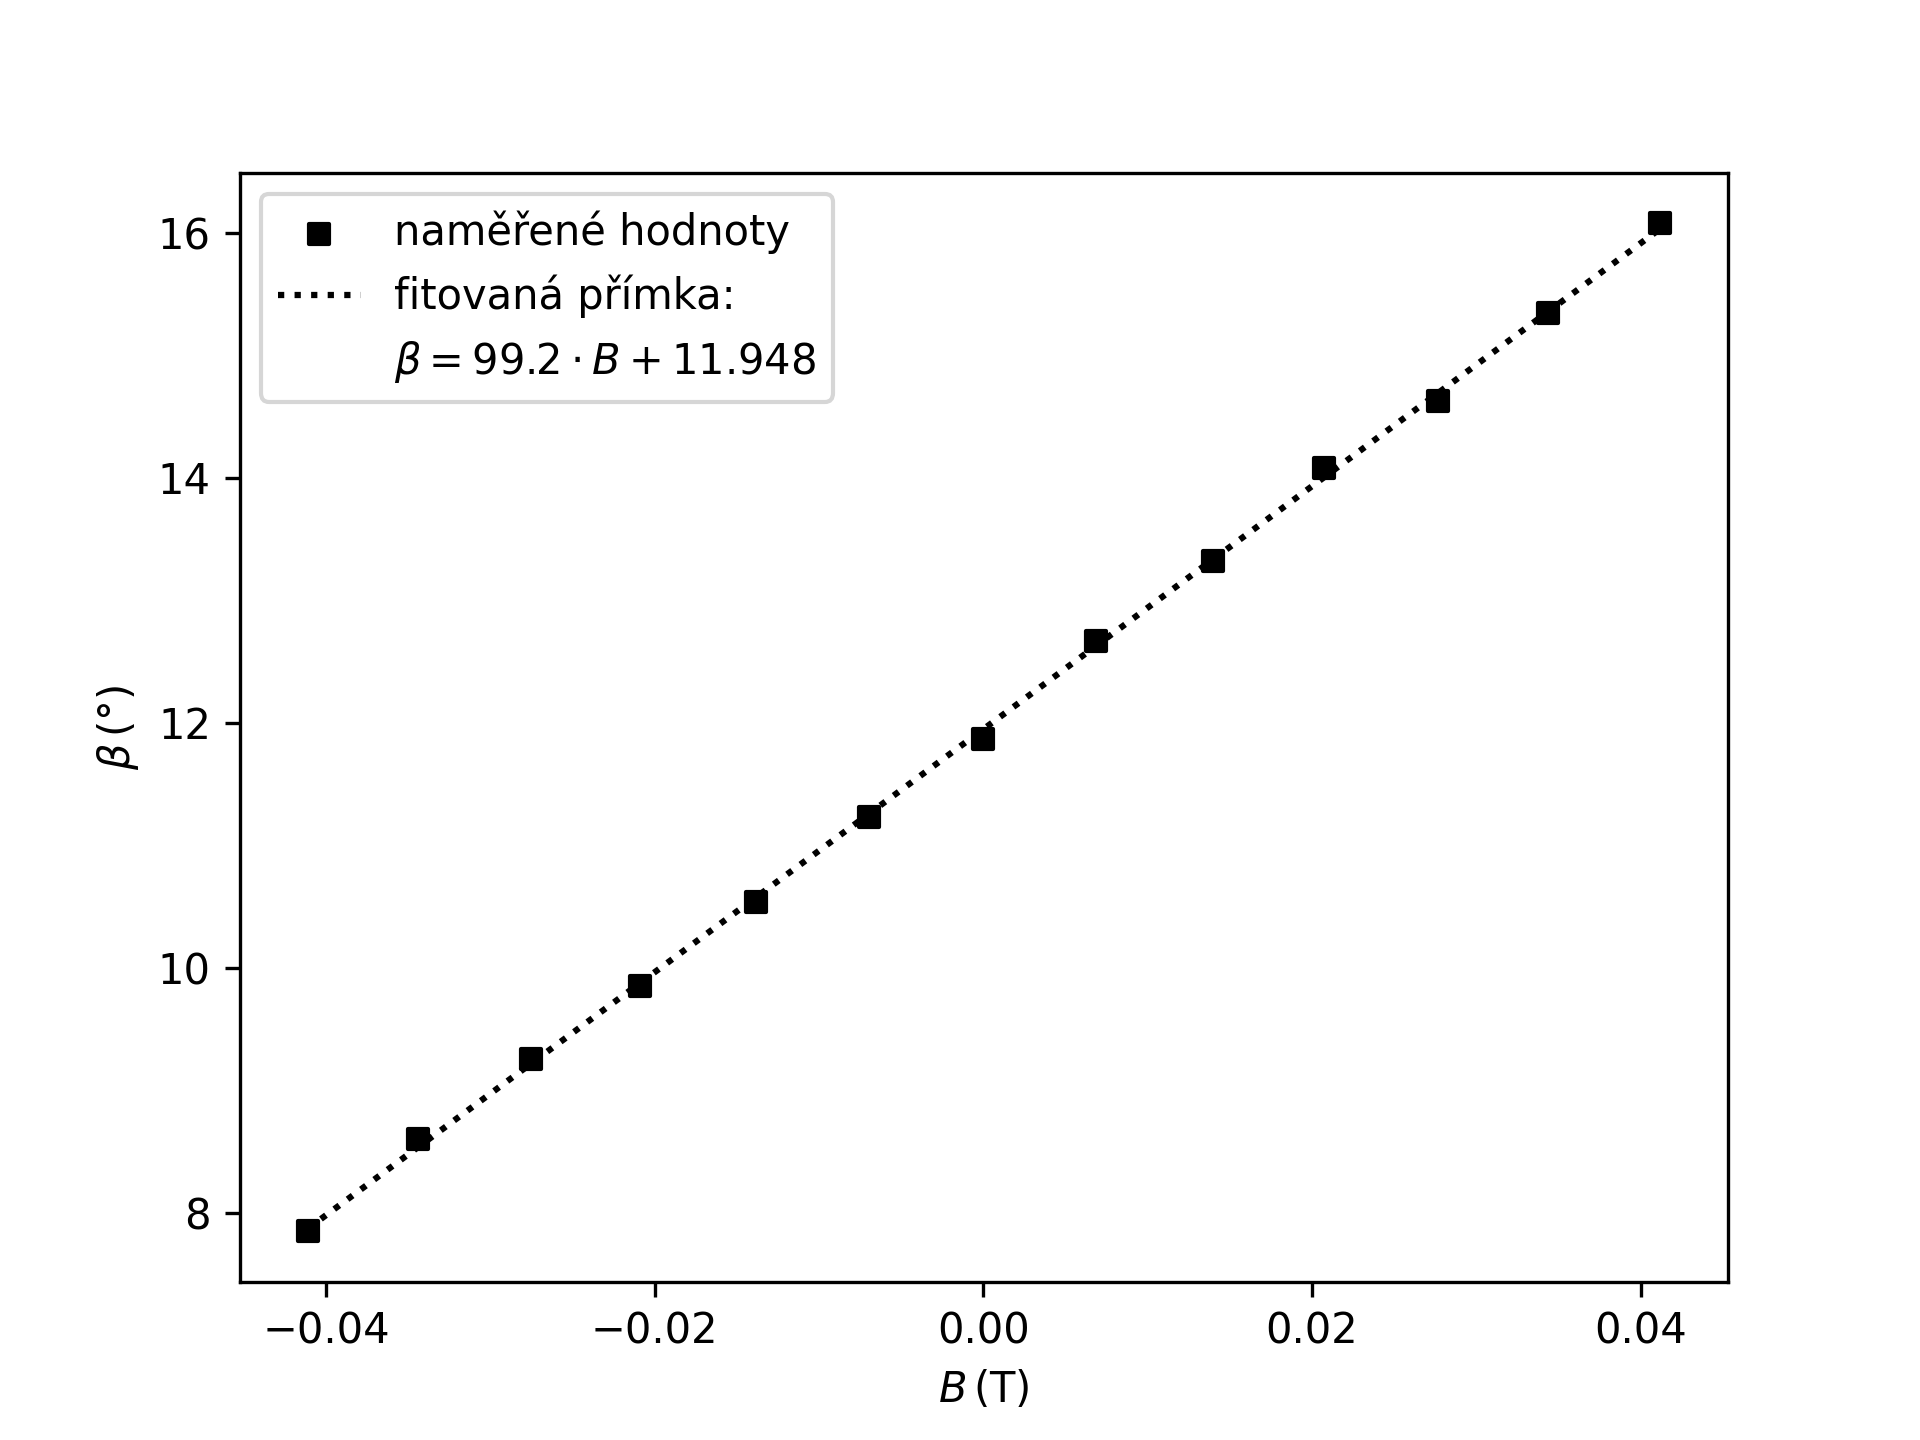
\includegraphics[width=0.5\linewidth]{benzen.png}
    \caption{Závislost úhlu $\beta$ na~stupnici polarimetru na~magnetické indukci solenoidu.\nobars}
    \label{fig:benzen}
\end{figure}



% ============================ DISKUZE ===============================
\section{Diskuze}

\textit{Měrná stáčivost roztoku glukózy.} Úhel stočení polarizační roviny byl měřen polostínovou metodou v~nastavení,
kdy jsou jasy obou polovin zorného pole blízko svého minima. Pozici, kdy jsou obě poloviny stejně jasné, lze takto
určit s~větší přesností, než v~blízkosti jejich maximálního jasu. Díky tomu, že se~světelné podmínky ani experimentátor 
během měření nezměnily,
lze přesnost určení úhlu polostínovou metodou změřit pro~jeden vzorek a~stejnou hodnotu přenést na~ostatní měření.
Pro~odhad skutečného vlivu nejistoty koncentrace na~úhel stočení byl vzorek o~koncentraci \qty{100}{g \per l} namíchán
třikrát. Nejistota koncentrace bude jistě daná nejistotou pipetovaného objemu glukózy, jež byl odhadnut z~dřívějšího měření,
avšak takto lze zohlednit např. i~nedokonalé promíchání roztoku, kdy by byla koncentrace v~jednom místě kádinky větší než~v~jiném.
Tímto postupem byla určena nejistota úhlu $\beta$ jako \qty{0.2}{\degree}.

Na~stupnici polarimetru nebyl měřen přímo úhel stočení $\alpha$, ten je dán rozdílem úhlu $\beta$ za~použití vzorku o~koncentraci
$c$ a~úhlu $\beta_0$ naměřeného pro~destilovanou vodu. Odečítáním těchto dvou úhlů se~však podle vztahu
(\ref{eq:sigma_alfa_glukoza}) zvětšuje nejistota úhlu stočení, která má kvůli své velikosti hlavní vliv na~nejistotu měrné
stáčivosti. Proto byla kromě prostého artimetického průměru měrných stáčivostí jednotlivých vzorků provedena i~lineární regrese
závislosti úhlu $\beta$ na~koncentraci (z~grafu \ref{fig:glukoza} je patrné, že úhel stočení je v~dobrém přiblížení lineárně 
závislý na~koncentraci vzorku a~lineární model má tedy dobrý smysl). 

Průměrováním měrných stáčivostí jednotlivých vzorků vychází hodnota $\overline{\rho} = \qty{0.052(2)}{\degree dm^{2} g^{-1}}$
s~relativní nejistotou $4\,\%$, zatímco z~lineární regrese $\tilde{\rho} = \qty{0.0525(5)}{ \degree dm^2 g^{-1} }$ s~relativní
nejistotou $1\,\%$. Obě měrné stáčivosti se~v~rámci nejistoty shodují, avšak hodnota z~lineární regrese je přesnější.
Pro~spektrální čáru sodíku D je v~uvedená hodnota měrné stáčivosti glukózy $\rho_{tab} = \qty{0.527}{\degree dm^2 g^{-1}}$
\cite{weast}, tedy experimentální hodnoty se~v~rámci nejistoty shodují s~tabulkovou hodnotou. Je však potřeba poznamenat,
že~experiment nebyl prováděn se~sodíkovou výbojkou, ale s~rtuťovou výbojkou s~filtrem propouštějícím spektrální čáru e
o~vlnové délce $\lambda_e = \qty{546.1}{\nano\meter}$, která je o~několik desítek nanometrů nižší než vlnová délka
$\lambda_D = \qty{589.3}{nm}$.

\textit{Verdetova konstanta benzenu.} K~určení Verdetovy konstanty benzenu byl využit Faradayův jev, přičemž byla proměřována
závislost úhlu stočení polarizační roviny na~magnetické indukci solenoidu. Indukce není v~celém objemu solenoidu konstantní,
avšak uvažuji, že pro~určení úhlu stočení lze využít její střední hodnotu, která je podle aproximativního vztahu 
(\ref{eq:indukce_na_proudu}) přímo úměrná proudu procházejícímu solenoidem. Pro~jednoduchost byla opět nejistota
úhlu odhadnuta na~základě opakovaných měření pro~tři různé proudy (\qty{-2}{A}, \qty{-1}{A} a~\qty{1}{A}) a následně byla přenesena
na~všechna ostatní měření. V tomto případě vyšla pro~všechny tři proudy stejná hodnota $\sigma_\beta = 0.03 \,\degree$,
není tedy nutné ji nějakým způsobem interpolovat a~extrapolovat pro~ostatní hodnoty proudu.

Při~určování Verdetovy konstanty hrála opět (podle vztahu (\ref{eq:sigma_verdet})) největší roli nejistota úhlu stočení,
neboť nejistota indukce byla vůči ní díky přesnému měření proudu zanedbatelná. Pro~všechna měření
vychází relativní nejistota v~rozsahu $1-6\,\%$, přičemž největší je pro~nízké hodnoty indukce,
kdy je úhel stočení $\alpha$ malý. Malá přesnost se~projevila na~průměrné hodnotě Verdetovy konstanty 
$\overline{V} = \qty{50(1)}{\degree T^{-1} dm^{-1}}$ (rel. nejistota $2\,\%$). Hodnota z~lineární regrese
$\tilde{V} = \qty{49.6(3)}{\degree T^{-1} dm^{-1}}$ vychází s~relativní nejistotou jen $0.6\,\%$, protože nedocházelo
ke~zvětšování chyby při~odečítání dvou blízkých úhlů. V~rámci nejistoty však se~obě hodnoty Verdetovy konstanty shodují.
Tabulky \cite{broz} uvádějí hodnotu $V_{tab} = \qty{50}{\degree T^{-1} dm^{-1}}$, jež je v~souladu s~experimentem.
Z~grafu \ref{fig:benzen} je zřejmé, že úhel stočení polarizační roviny je skutečně lineárně závislý na~magnetické indukci.

% ============================= ZÁVĚR ================================ asi hotovo
\section{Závěr}

Měrná stáčivost glukózy pro~vlnovou délku \qty{546.1}{nm} byla určena průměrováním hodnot pro~jednotlivé roztoky
o~různých koncentracích jako $\overline{\rho} = \qty{0.052(2)}{\degree dm^{2} g^{-1}}$. Metodou nejmenších čtverců
z~lineární závislosti úhlu stočení na~koncentraci vychází hodnota
$\tilde{\rho} = \qty{0.0525(5)}{ \degree dm^2 g^{-1} }$.

Verdetova konstanta benzenu pro~vlnovou délku \qty{589.3}{nm} byla určena průměrováním hodnot pro~jednotlivé
hodnoty magnetické indukce jako $\overline{V} = \qty{50(1)}{\degree T^{-1} dm^{-1}}$. Z~metody nejmenších čtverců lineární 
závislosti úhlu stočení na~magnetické indukci vychází hodnota
$\tilde{V} = \qty{49.6(3)}{\degree T^{-1} dm^{-1}}$.


% =========================== LITERATURA =============================
\begin{thebibliography}{9}

\bibitem{studijni} Kolektiv ZFP KVOF MFF UK: \textit{Úloha 11 - studijní text} [online]. 
[cit. \today], dostupné z~https://physics.mff.cuni.cz/vyuka/zfp/\_media/zadani/texty/txt\_323.pdf

\bibitem{pokyny} Kolektiv ZFP KVOF MFF UK: \textit{Úloha 11 - pokyny k měření} [online]. [cit. \today], dostupné
z~https://physics.mff.cuni.cz/vyuka/zfp/\_media/zadani/pokyny/mereni\_311.pdf

\bibitem{vlnovedelky} Kolektiv ZFP KVOF MFF UK: \textit{Úloha 16 - studijní text} 
[online]. [cit. \today], dostupné
z~https://physics.mff.cuni.cz/vyuka/zfp/\_media/zadani/texty/txt\_316.pdf

\bibitem{englich} J. Englich: \textit{Úvod do praktické fyziky I: Zpracování výsledků měření}. 
1. vyd. Praha: Matfyzpress, 2006

\bibitem{weast} R. C. Weast (1974). \textit{Handbook of Chemistry and Physics} (55th ed.). CRC Press.

\bibitem{broz} BROŽ, Jaromír; ROSKOVEC, Vladimír a VALOUCH, Miloslav. \textit{Fyzikální a~matematické tabulky}. 
Praha:~Státní nakladatelství technické literatury, 1980.

% \bibitem{mikulcak} Mikulčák a kolektiv: \textit{Matematické, fyzikální a~chemické tabulky pro~střední 
% školy: NÁZEVTABULKY}, Praha: Státní pedagogické nakladatelství, n. p., 1988

\end{thebibliography}
\end{document}